\documentclass[]{article}
\usepackage{lmodern}
\usepackage{amssymb,amsmath}
\usepackage{ifxetex,ifluatex}
\usepackage{fixltx2e} % provides \textsubscript
\ifnum 0\ifxetex 1\fi\ifluatex 1\fi=0 % if pdftex
  \usepackage[T1]{fontenc}
  \usepackage[utf8]{inputenc}
\else % if luatex or xelatex
  \ifxetex
    \usepackage{mathspec}
  \else
    \usepackage{fontspec}
  \fi
  \defaultfontfeatures{Ligatures=TeX,Scale=MatchLowercase}
\fi
% use upquote if available, for straight quotes in verbatim environments
\IfFileExists{upquote.sty}{\usepackage{upquote}}{}
% use microtype if available
\IfFileExists{microtype.sty}{%
\usepackage{microtype}
\UseMicrotypeSet[protrusion]{basicmath} % disable protrusion for tt fonts
}{}
\usepackage[margin=1in]{geometry}
\usepackage{hyperref}
\hypersetup{unicode=true,
            pdftitle={\#TidyTuesday: Which are the best family cars for your weekend trip?},
            pdfborder={0 0 0},
            breaklinks=true}
\urlstyle{same}  % don't use monospace font for urls
\usepackage{color}
\usepackage{fancyvrb}
\newcommand{\VerbBar}{|}
\newcommand{\VERB}{\Verb[commandchars=\\\{\}]}
\DefineVerbatimEnvironment{Highlighting}{Verbatim}{commandchars=\\\{\}}
% Add ',fontsize=\small' for more characters per line
\usepackage{framed}
\definecolor{shadecolor}{RGB}{248,248,248}
\newenvironment{Shaded}{\begin{snugshade}}{\end{snugshade}}
\newcommand{\AlertTok}[1]{\textcolor[rgb]{0.94,0.16,0.16}{#1}}
\newcommand{\AnnotationTok}[1]{\textcolor[rgb]{0.56,0.35,0.01}{\textbf{\textit{#1}}}}
\newcommand{\AttributeTok}[1]{\textcolor[rgb]{0.77,0.63,0.00}{#1}}
\newcommand{\BaseNTok}[1]{\textcolor[rgb]{0.00,0.00,0.81}{#1}}
\newcommand{\BuiltInTok}[1]{#1}
\newcommand{\CharTok}[1]{\textcolor[rgb]{0.31,0.60,0.02}{#1}}
\newcommand{\CommentTok}[1]{\textcolor[rgb]{0.56,0.35,0.01}{\textit{#1}}}
\newcommand{\CommentVarTok}[1]{\textcolor[rgb]{0.56,0.35,0.01}{\textbf{\textit{#1}}}}
\newcommand{\ConstantTok}[1]{\textcolor[rgb]{0.00,0.00,0.00}{#1}}
\newcommand{\ControlFlowTok}[1]{\textcolor[rgb]{0.13,0.29,0.53}{\textbf{#1}}}
\newcommand{\DataTypeTok}[1]{\textcolor[rgb]{0.13,0.29,0.53}{#1}}
\newcommand{\DecValTok}[1]{\textcolor[rgb]{0.00,0.00,0.81}{#1}}
\newcommand{\DocumentationTok}[1]{\textcolor[rgb]{0.56,0.35,0.01}{\textbf{\textit{#1}}}}
\newcommand{\ErrorTok}[1]{\textcolor[rgb]{0.64,0.00,0.00}{\textbf{#1}}}
\newcommand{\ExtensionTok}[1]{#1}
\newcommand{\FloatTok}[1]{\textcolor[rgb]{0.00,0.00,0.81}{#1}}
\newcommand{\FunctionTok}[1]{\textcolor[rgb]{0.00,0.00,0.00}{#1}}
\newcommand{\ImportTok}[1]{#1}
\newcommand{\InformationTok}[1]{\textcolor[rgb]{0.56,0.35,0.01}{\textbf{\textit{#1}}}}
\newcommand{\KeywordTok}[1]{\textcolor[rgb]{0.13,0.29,0.53}{\textbf{#1}}}
\newcommand{\NormalTok}[1]{#1}
\newcommand{\OperatorTok}[1]{\textcolor[rgb]{0.81,0.36,0.00}{\textbf{#1}}}
\newcommand{\OtherTok}[1]{\textcolor[rgb]{0.56,0.35,0.01}{#1}}
\newcommand{\PreprocessorTok}[1]{\textcolor[rgb]{0.56,0.35,0.01}{\textit{#1}}}
\newcommand{\RegionMarkerTok}[1]{#1}
\newcommand{\SpecialCharTok}[1]{\textcolor[rgb]{0.00,0.00,0.00}{#1}}
\newcommand{\SpecialStringTok}[1]{\textcolor[rgb]{0.31,0.60,0.02}{#1}}
\newcommand{\StringTok}[1]{\textcolor[rgb]{0.31,0.60,0.02}{#1}}
\newcommand{\VariableTok}[1]{\textcolor[rgb]{0.00,0.00,0.00}{#1}}
\newcommand{\VerbatimStringTok}[1]{\textcolor[rgb]{0.31,0.60,0.02}{#1}}
\newcommand{\WarningTok}[1]{\textcolor[rgb]{0.56,0.35,0.01}{\textbf{\textit{#1}}}}
\usepackage{graphicx,grffile}
\makeatletter
\def\maxwidth{\ifdim\Gin@nat@width>\linewidth\linewidth\else\Gin@nat@width\fi}
\def\maxheight{\ifdim\Gin@nat@height>\textheight\textheight\else\Gin@nat@height\fi}
\makeatother
% Scale images if necessary, so that they will not overflow the page
% margins by default, and it is still possible to overwrite the defaults
% using explicit options in \includegraphics[width, height, ...]{}
\setkeys{Gin}{width=\maxwidth,height=\maxheight,keepaspectratio}
\IfFileExists{parskip.sty}{%
\usepackage{parskip}
}{% else
\setlength{\parindent}{0pt}
\setlength{\parskip}{6pt plus 2pt minus 1pt}
}
\setlength{\emergencystretch}{3em}  % prevent overfull lines
\providecommand{\tightlist}{%
  \setlength{\itemsep}{0pt}\setlength{\parskip}{0pt}}
\setcounter{secnumdepth}{0}
% Redefines (sub)paragraphs to behave more like sections
\ifx\paragraph\undefined\else
\let\oldparagraph\paragraph
\renewcommand{\paragraph}[1]{\oldparagraph{#1}\mbox{}}
\fi
\ifx\subparagraph\undefined\else
\let\oldsubparagraph\subparagraph
\renewcommand{\subparagraph}[1]{\oldsubparagraph{#1}\mbox{}}
\fi

%%% Use protect on footnotes to avoid problems with footnotes in titles
\let\rmarkdownfootnote\footnote%
\def\footnote{\protect\rmarkdownfootnote}

%%% Change title format to be more compact
\usepackage{titling}

% Create subtitle command for use in maketitle
\providecommand{\subtitle}[1]{
  \posttitle{
    \begin{center}\large#1\end{center}
    }
}

\setlength{\droptitle}{-2em}

  \title{\#TidyTuesday: Which are the best family cars for your weekend trip?}
    \pretitle{\vspace{\droptitle}\centering\huge}
  \posttitle{\par}
    \author{}
    \preauthor{}\postauthor{}
      \predate{\centering\large\emph}
  \postdate{\par}
    \date{2019-10-23}


\begin{document}
\maketitle

This week, I will analyze Car Fuel Economy
\href{https://github.com/rfordatascience/tidytuesday/tree/master/data/2019/2019-10-15}{dataset}
from TidyTuesday.

\hypertarget{what-is-tidytuesday}{%
\subsection{What is TidyTuesday?}\label{what-is-tidytuesday}}

TidyTuesday is a weekly social data project in R organized by the
\href{https://thomasmock.netlify.com/post/tidytuesday-a-weekly-social-data-project-in-r/}{R
for Data Science community}.

It is a great way of improving your Data wrangling and visualization
techniques, \textbf{sharing and learning from others}.

You can find all the information on
\href{https://github.com/rfordatascience/tidytuesday}{github}.

Fuel economy \href{https://www.fueleconomy.gov/feg/download.shtml}{data}
are the result of the work done by the US Environmental Protection
Agency. Full data dictionary can be found at
\href{https://www.fueleconomy.gov/feg/ws/index.shtml\#fuelType1}{fueleconomy.gov}.

The data contains information of 83 parameters of more than 40.000
Vehicles. That's a lot of information!

\hypertarget{going-for-your-next-family-camping-adventure-first-check-your-car-model.}{%
\section{Going for your next family camping adventure? First, check your
car
model.}\label{going-for-your-next-family-camping-adventure-first-check-your-car-model.}}

Better Fuel economy and recent developments on longer running electric
car batteries are great but one thing which does not change in families'
lives is the \textbf{need for space}.

If you don't want crying kids running around because of \textbf{a
missing teddy bear} which did not fit in the baggage. Check, which
brands will serve you best.

Especially, if you have a daughter who likes to travel with a lot of
toys.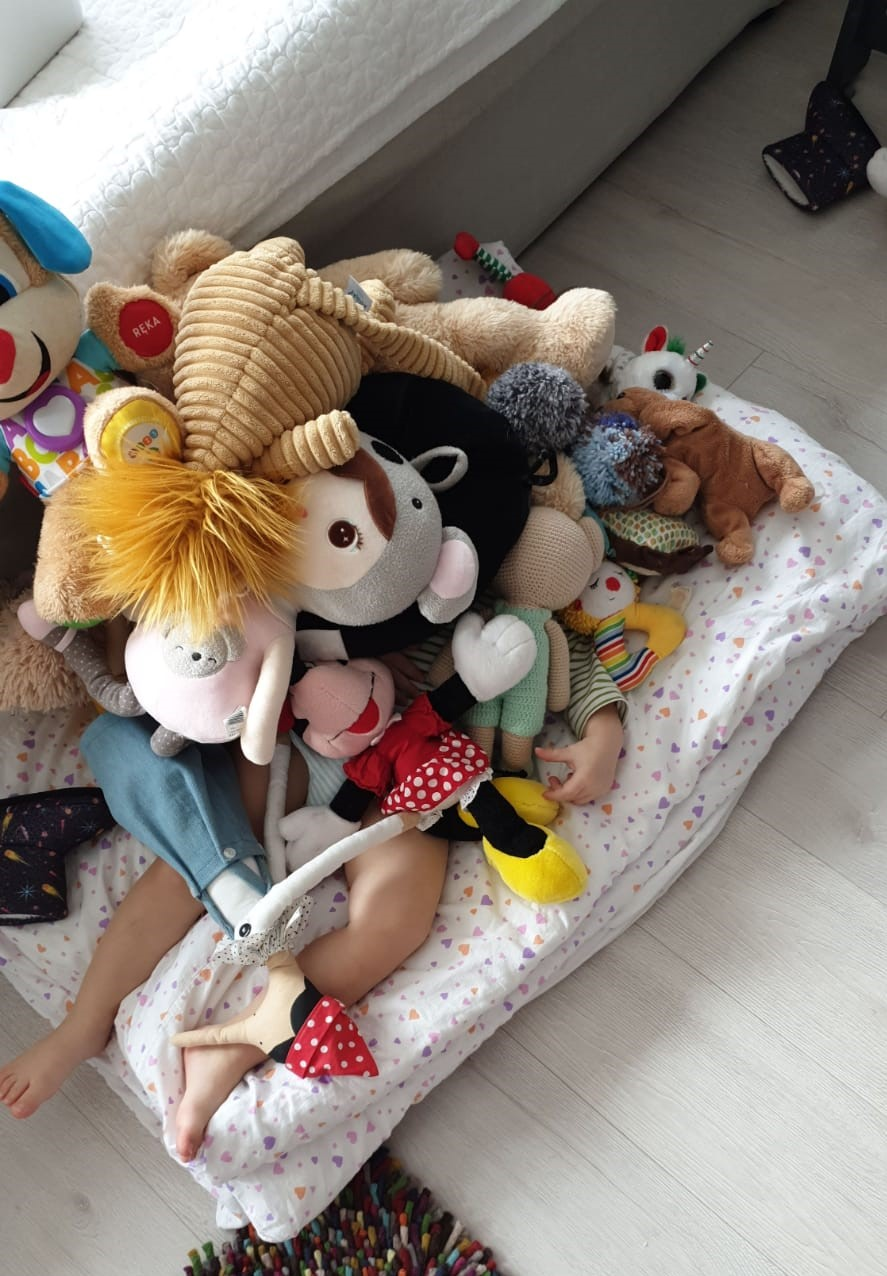
\includegraphics{/img/raisa.jpg}\\
Let's figure out a solution for peaceful weekend trip.

\hypertarget{which-brand-produce-most-family-friendly-cars-in-terms-of-baggage-volume.}{%
\section{Which brand produce most family friendly cars? In terms of
baggage
volume.}\label{which-brand-produce-most-family-friendly-cars-in-terms-of-baggage-volume.}}

\begin{Shaded}
\begin{Highlighting}[]
\KeywordTok{library}\NormalTok{(tidyverse) }\CommentTok{# ggplot2, dplyr, tidyr, readr, }
                   \CommentTok{# purrr, tibble, stringr, forcats}
\NormalTok{big_epa_cars <-}\StringTok{ }\KeywordTok{read_csv}\NormalTok{(}\StringTok{"https://raw.githubusercontent.com/rfordatascience/tidytuesday/master/data/2019/2019-10-15/big_epa_cars.csv"}\NormalTok{)}
\KeywordTok{dim}\NormalTok{(big_epa_cars)}
\end{Highlighting}
\end{Shaded}

\begin{verbatim}
## [1] 41804    83
\end{verbatim}

I will subset my data for easier computation

Let's keep the following columns:

\begin{itemize}
\tightlist
\item
  year - model year
\item
  make - manufacturer (division)
\item
  model - model name (carline)
\item
  VClass - EPA vehicle size class
\item
  hlv - hatchback luggage volume (cubic feet)
\item
  hpv - hatchback passenger volume (cubic feet)
\item
  displ - engine displacement in liters
\item
  lv4 - 4 door luggage volume (cubic feet)
\item
  pv4 - 4-door passenger volume
\end{itemize}

\begin{Shaded}
\begin{Highlighting}[]
\NormalTok{big_sub <-}\StringTok{ }\NormalTok{big_epa_cars }\OperatorTok\StringTok{ }
\StringTok{  }\KeywordTok{select}\NormalTok{(fuelType, year, make, model, VClass, hlv, hpv,lv4,pv4,displ)}
\end{Highlighting}
\end{Shaded}

I will start exploring the data. For the moment, first I will focus on
Midsize cars (VClass)

I will filter for the main pool of Midsize cars with 4 door and luggage
volume of bigger than 6 and passenger volume larger than 75.

\begin{Shaded}
\begin{Highlighting}[]
\NormalTok{posn.j <-}\StringTok{ }\KeywordTok{position_jitter}\NormalTok{(}\DataTypeTok{width=}\FloatTok{0.2}\NormalTok{)}
\NormalTok{big_sw <-}\StringTok{ }\NormalTok{big_sub }\OperatorTok\StringTok{ }
\StringTok{  }\KeywordTok{filter}\NormalTok{(VClass }\OperatorTok{==}\StringTok{ "Midsize Cars"} \OperatorTok{&}\StringTok{ }\NormalTok{pv4 }\OperatorTok{>}\StringTok{ }\DecValTok{75} \OperatorTok{&}\StringTok{ }\NormalTok{lv4 }\OperatorTok{>}\StringTok{ }\DecValTok{6}\NormalTok{) }

\NormalTok{big_sw }\OperatorTok
\StringTok{  }\KeywordTok{ggplot}\NormalTok{(}\KeywordTok{aes}\NormalTok{(}\DataTypeTok{x=}\NormalTok{pv4, }\DataTypeTok{y=}\NormalTok{lv4)) }\OperatorTok{+}\StringTok{ }
\StringTok{  }\KeywordTok{geom_point}\NormalTok{(}\DataTypeTok{shape=}\DecValTok{21}\NormalTok{, }\DataTypeTok{alpha=}\FloatTok{0.4}\NormalTok{,}\DataTypeTok{size =}\DecValTok{3}\NormalTok{, }\DataTypeTok{position =}\NormalTok{ posn.j) }\OperatorTok{+}\StringTok{ }
\StringTok{  }\KeywordTok{theme}\NormalTok{(}\DataTypeTok{plot.caption=}\KeywordTok{element_text}\NormalTok{(}\DataTypeTok{size=}\DecValTok{11}\NormalTok{), }\DataTypeTok{text =} \KeywordTok{element_text}\NormalTok{(}\DataTypeTok{size=}\DecValTok{18}\NormalTok{),    }\DataTypeTok{plot.title =} \KeywordTok{element_text}\NormalTok{(}\DataTypeTok{size=}\DecValTok{32}\NormalTok{), }\DataTypeTok{legend.position =} \StringTok{"none"}\NormalTok{) }\OperatorTok{+}
\StringTok{  }\KeywordTok{geom_smooth}\NormalTok{(}\DataTypeTok{method =} \StringTok{"lm"}\NormalTok{, }\DataTypeTok{color =}\StringTok{"red"}\NormalTok{) }\OperatorTok{+}\StringTok{ }
\StringTok{  }\KeywordTok{coord_fixed}\NormalTok{() }\OperatorTok{+}
\StringTok{    }\KeywordTok{labs}\NormalTok{(}\DataTypeTok{x =} \StringTok{"Passenger Vol (Cubic feet)"}\NormalTok{, }\DataTypeTok{y =} \StringTok{"Luggage Vol (Cubic feet)"}\NormalTok{, }\DataTypeTok{title =} \StringTok{"Luggage space negatively }\CharTok{\textbackslash{}n}\StringTok{correlates with passenger space"}\NormalTok{)}
\end{Highlighting}
\end{Shaded}

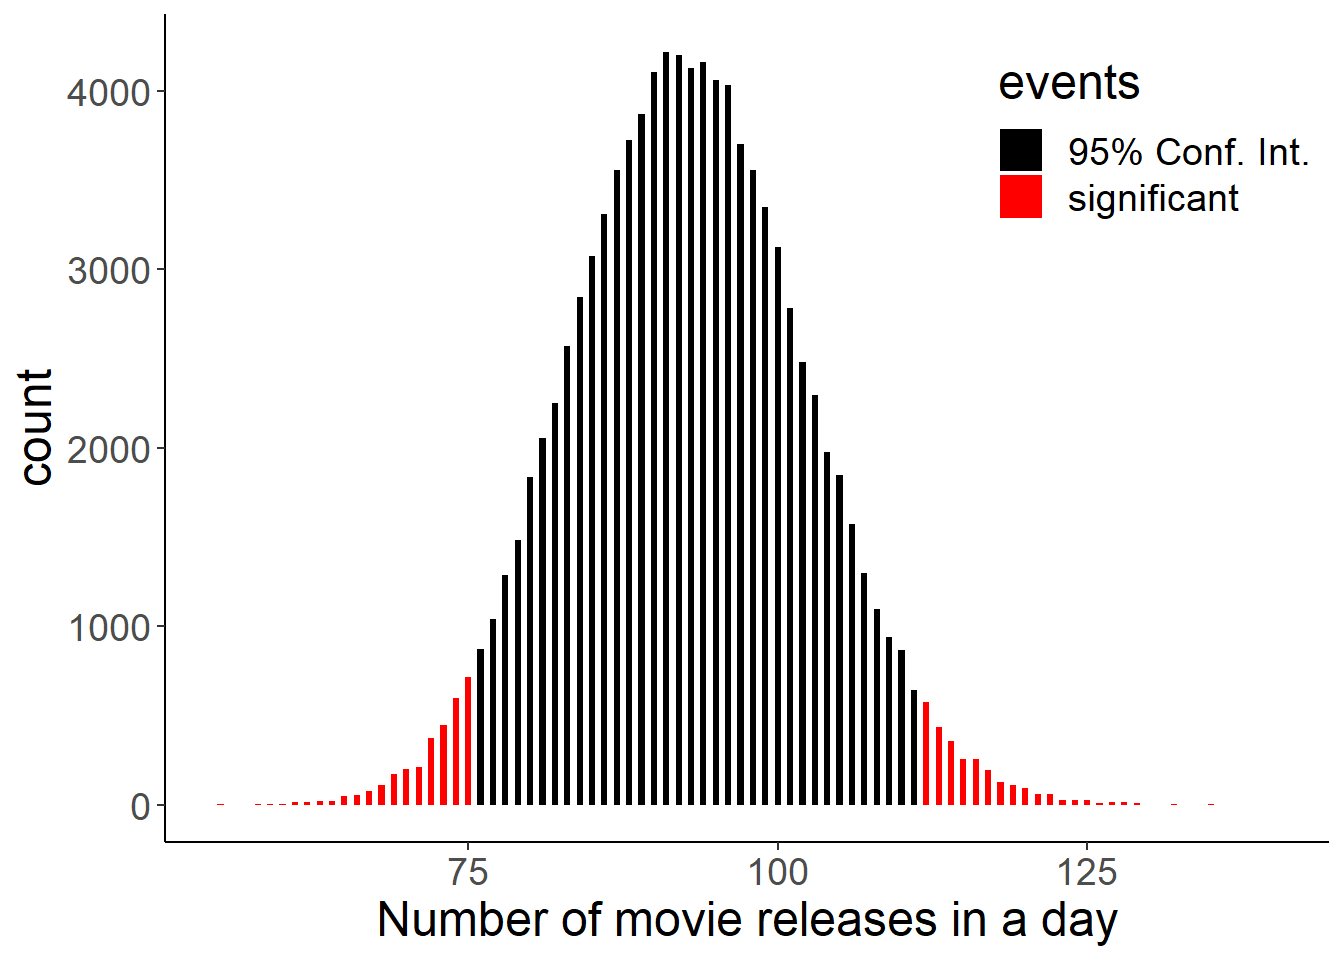
\includegraphics{2019-10-23-tidytuesday-which-are-the-best-family-cars_files/figure-latex/unnamed-chunk-2-1.pdf}

This is not unexpected. But good to see.

\begin{quote}
Insight 1: Negative correlation suggests that producers sacrifice
passenger space to produce bigger room for the luggage or vice versa.
\end{quote}

First, I will look at the luggage volume in Mid sized cars and I will
order them according to highest average.

\begin{Shaded}
\begin{Highlighting}[]
\NormalTok{pp <-}\StringTok{ }\NormalTok{big_sw }\OperatorTok\StringTok{ }
\StringTok{  }\KeywordTok{mutate}\NormalTok{(}\DataTypeTok{make =} \KeywordTok{fct_reorder}\NormalTok{(make, lv4)) }\OperatorTok
\StringTok{  }\KeywordTok{ggplot}\NormalTok{(}\KeywordTok{aes}\NormalTok{(}\DataTypeTok{x=}\NormalTok{make, }\DataTypeTok{y=}\NormalTok{lv4, }\DataTypeTok{col=}\NormalTok{make)) }\OperatorTok{+}\StringTok{ }
\StringTok{  }\KeywordTok{geom_boxplot}\NormalTok{(}\DataTypeTok{varwidth=}\OtherTok{TRUE}\NormalTok{) }\OperatorTok{+}
\StringTok{  }\KeywordTok{theme}\NormalTok{(}\DataTypeTok{plot.caption=}\KeywordTok{element_text}\NormalTok{(}\DataTypeTok{size=}\DecValTok{11}\NormalTok{), }\DataTypeTok{text =} \KeywordTok{element_text}\NormalTok{(}\DataTypeTok{size=}\DecValTok{18}\NormalTok{),    }\DataTypeTok{plot.title =} \KeywordTok{element_text}\NormalTok{(}\DataTypeTok{size=}\DecValTok{32}\NormalTok{), }\DataTypeTok{legend.position =} \StringTok{"none"}\NormalTok{) }\OperatorTok{+}
\StringTok{  }\KeywordTok{coord_flip}\NormalTok{() }\OperatorTok{+}\StringTok{ }
\StringTok{  }\KeywordTok{labs}\NormalTok{(}\DataTypeTok{x =} \KeywordTok{element_blank}\NormalTok{(), }\DataTypeTok{y =} \StringTok{"Luggage size (cubic feet)"}\NormalTok{, }\DataTypeTok{title =} \StringTok{"Average luggage volumes in Midsized cars"}\NormalTok{)}
\NormalTok{  pp}
\end{Highlighting}
\end{Shaded}

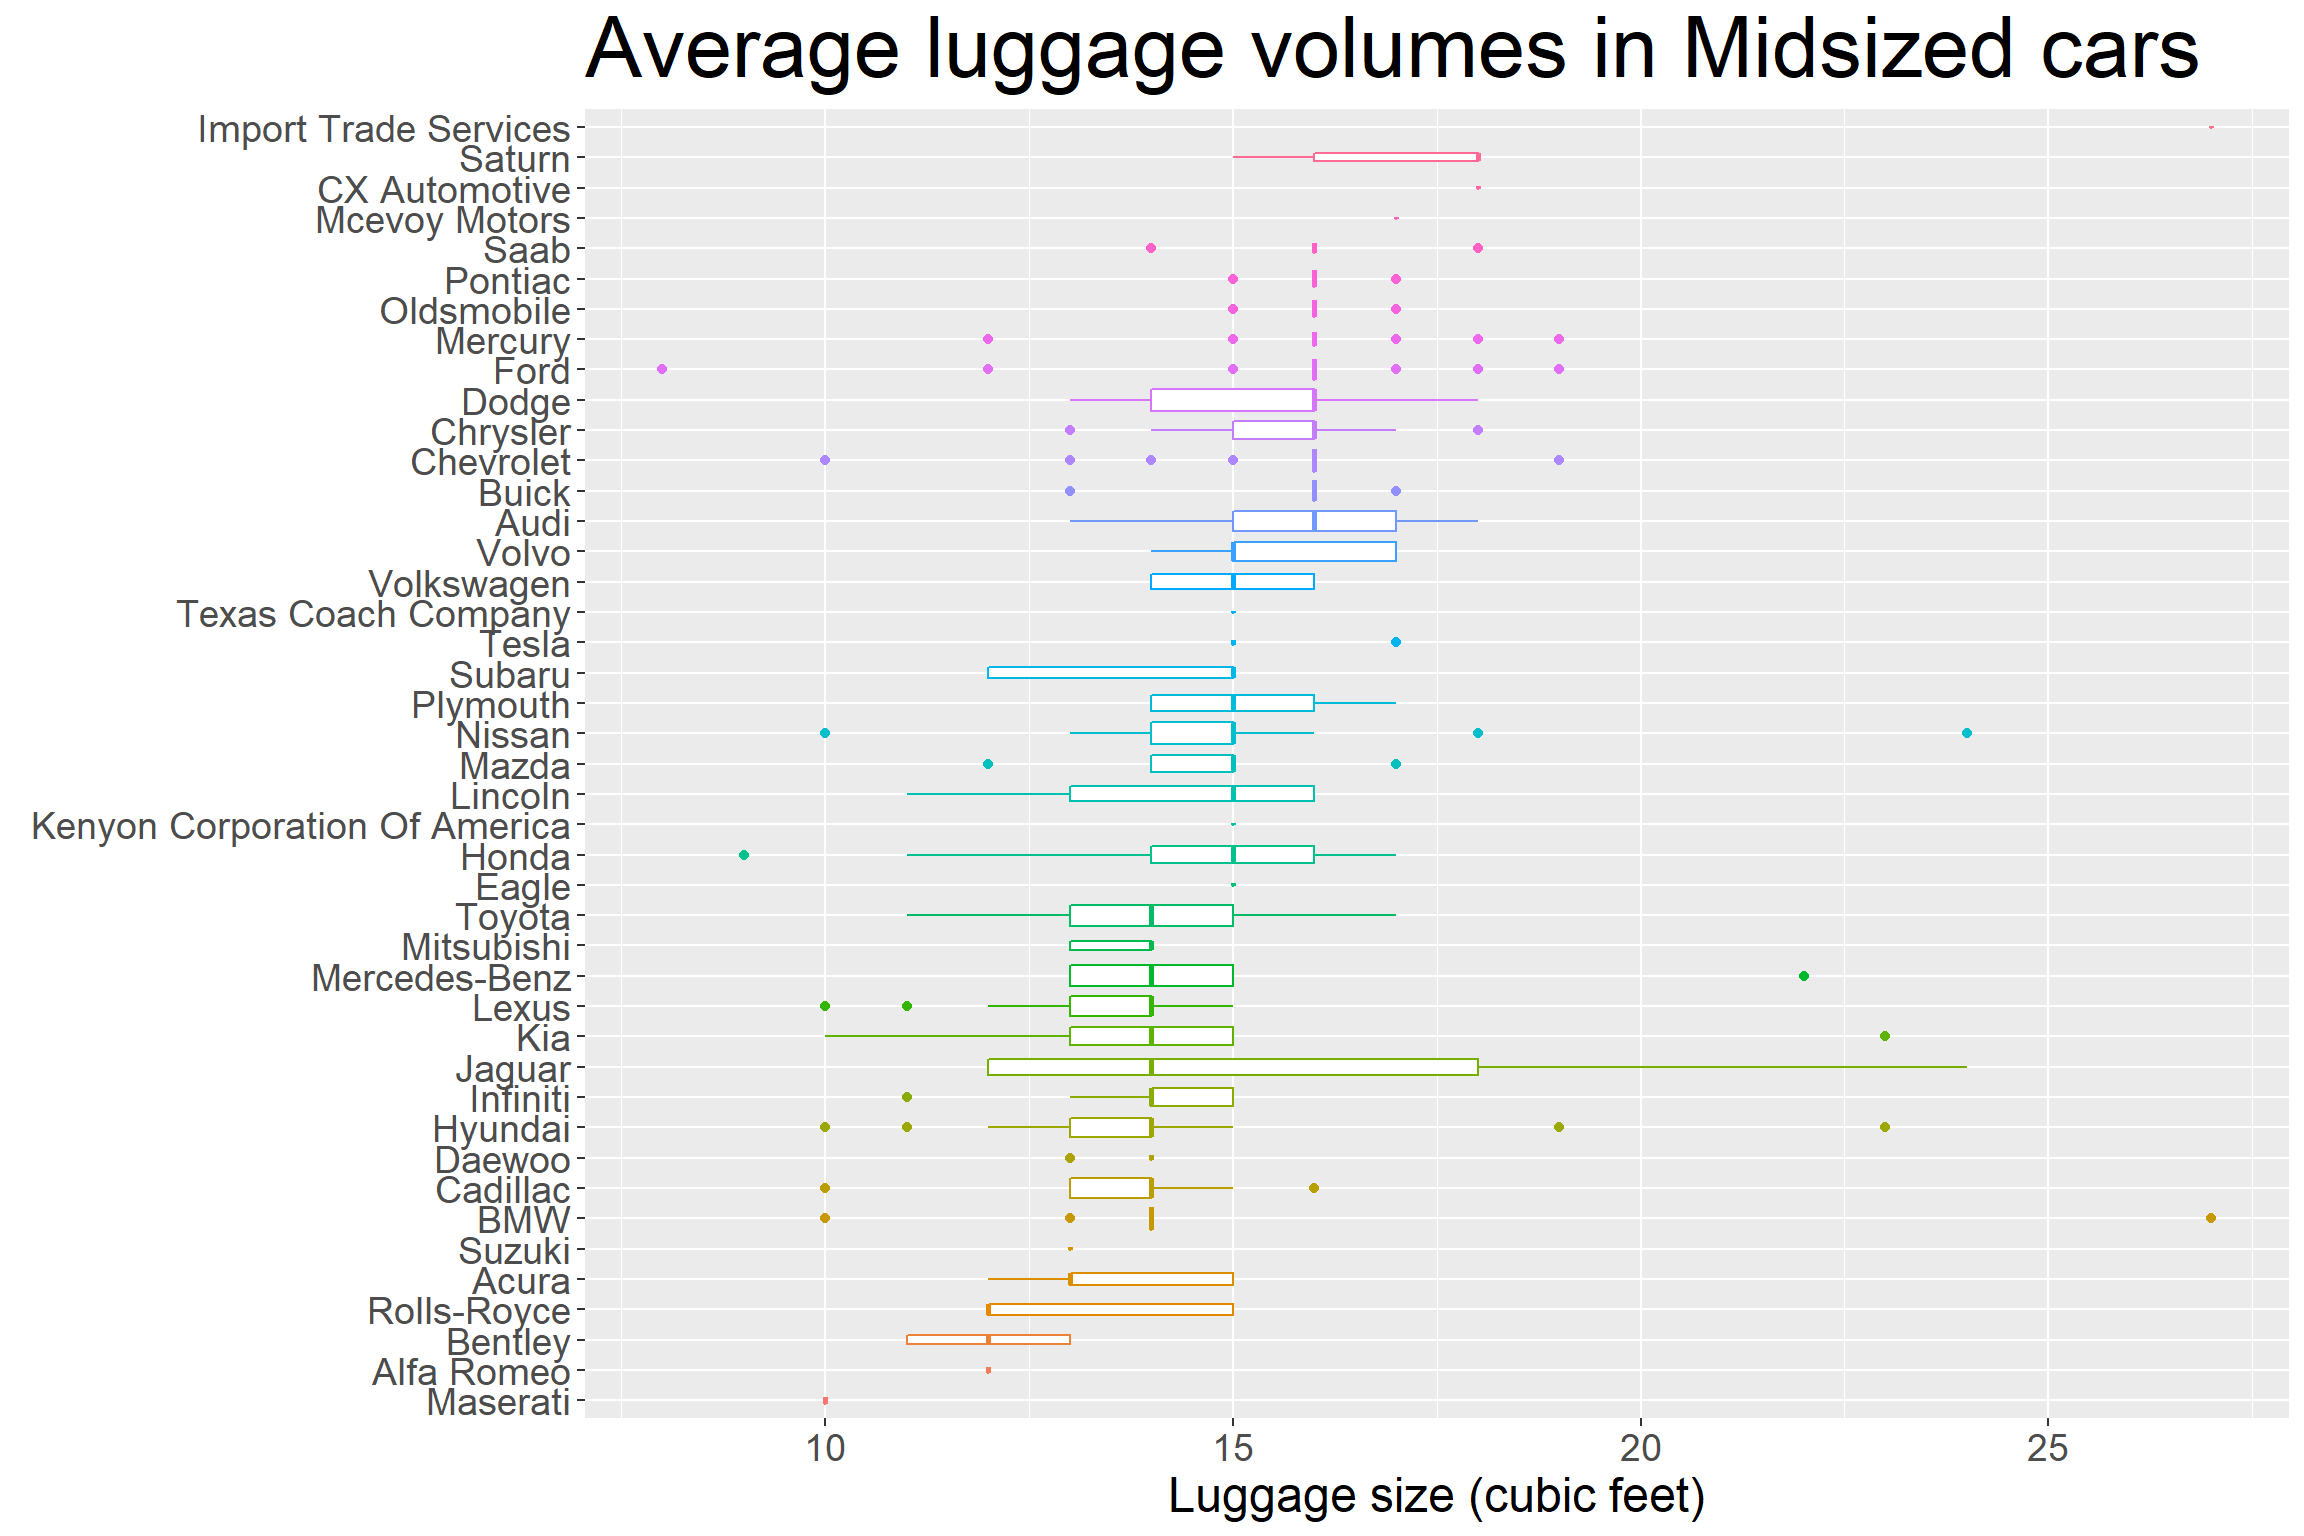
\includegraphics{2019-10-23-tidytuesday-which-are-the-best-family-cars_files/figure-latex/unnamed-chunk-3-1.pdf}

If you follow the mean lines from bottom to top, you will see that cars
cluster into three groups according to their mean of luggage sizes. But
differences are not huge.

\begin{quote}
Insight 2: Cars cluster into three groups according to their mean
luggage size.
\end{quote}

Let's focus. I am looking for the car with the biggest luggage space.
Let's see what other VClass types are in our dataset that we can include
our exploration.

There are 34 types of vehicle classes (Vlass) in our dataset. I will
subset all the relevant ones, leaving some specialty vehicles and vans
aside.

You can have a look at other VClass types with this code here.

\texttt{big\_epa\_cars\ \%\textgreater{}\%\ group\_by(VClass)\ \%\textgreater{}\%\ count()\ \%\textgreater{}\%\ arrange(desc(n))}

I will also remove minor brands with less than 10 models in total.

\begin{Shaded}
\begin{Highlighting}[]
\NormalTok{big_filtered <-}\StringTok{ }\NormalTok{big_sub }\OperatorTok\StringTok{ }
\StringTok{  }\KeywordTok{filter}\NormalTok{(VClass }\OperatorTok\StringTok{ }\KeywordTok{c}\NormalTok{(}\StringTok{"Large Cars"}\NormalTok{, }\StringTok{"Compact Cars"}\NormalTok{, }\StringTok{"Midsize Cars"}\NormalTok{, }
                       \StringTok{"Midsize Station Wagons"}\NormalTok{, }\StringTok{"Midsize-Large Station Wagons"}\NormalTok{,}
                       \StringTok{"Minivan - 2WD"}\NormalTok{, }\StringTok{"Minivan - 4WD"}\NormalTok{)) }\OperatorTok\StringTok{ }
\StringTok{  }\KeywordTok{group_by}\NormalTok{(make) }\OperatorTok\StringTok{ }
\StringTok{  }\KeywordTok{mutate}\NormalTok{(}\DataTypeTok{n=}\KeywordTok{n}\NormalTok{()) }\OperatorTok\StringTok{ }
\StringTok{  }\KeywordTok{filter}\NormalTok{(n }\OperatorTok{>}\StringTok{ }\DecValTok{10}\NormalTok{) }\OperatorTok\StringTok{ }
\StringTok{  }\KeywordTok{ungroup}\NormalTok{()}

\KeywordTok{dim}\NormalTok{(big_filtered)}
\end{Highlighting}
\end{Shaded}

\begin{verbatim}
## [1] 14710    11
\end{verbatim}

To be on the safe side for the family trip, I will choose cars not older
than 5 years.

\begin{Shaded}
\begin{Highlighting}[]
\CommentTok{# Cars ordered with luggage volume, but not older than 5 years }
\CommentTok{# and lv4 bigger than 5}

\NormalTok{q <-}\StringTok{ }\NormalTok{big_filtered }\OperatorTok\StringTok{ }
\StringTok{  }\KeywordTok{filter}\NormalTok{(year }\OperatorTok{>}\StringTok{ }\DecValTok{2016}\NormalTok{, lv4 }\OperatorTok{>}\StringTok{ }\DecValTok{5}\NormalTok{) }\OperatorTok
\StringTok{  }\KeywordTok{mutate}\NormalTok{(}\DataTypeTok{make =} \KeywordTok{fct_reorder}\NormalTok{(make, lv4)) }\OperatorTok
\StringTok{  }\KeywordTok{ggplot}\NormalTok{(}\KeywordTok{aes}\NormalTok{(}\DataTypeTok{x=}\NormalTok{make, }\DataTypeTok{y=}\NormalTok{lv4, }\DataTypeTok{col=}\NormalTok{make)) }\OperatorTok{+}\StringTok{ }
\StringTok{  }\KeywordTok{geom_boxplot}\NormalTok{(}\DataTypeTok{varwidth=}\OtherTok{TRUE}\NormalTok{) }\OperatorTok{+}
\StringTok{  }\KeywordTok{theme}\NormalTok{(}\DataTypeTok{text =} \KeywordTok{element_text}\NormalTok{(}\DataTypeTok{size=}\DecValTok{15}\NormalTok{), }\DataTypeTok{legend.position =} \StringTok{"none"}\NormalTok{) }\OperatorTok{+}
\StringTok{  }\KeywordTok{coord_flip}\NormalTok{()}
\NormalTok{q}
\end{Highlighting}
\end{Shaded}

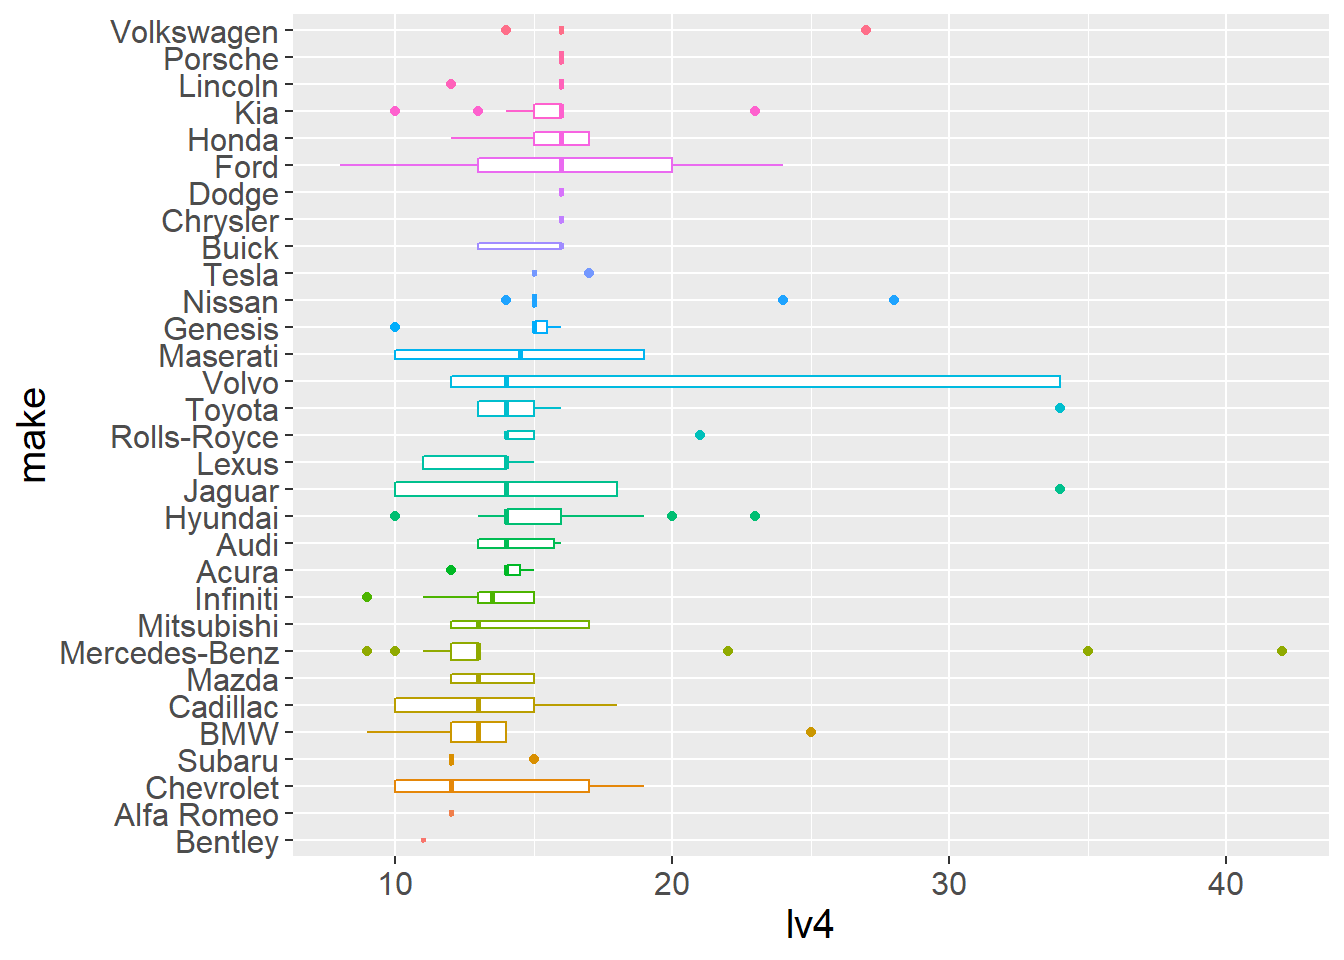
\includegraphics{2019-10-23-tidytuesday-which-are-the-best-family-cars_files/figure-latex/unnamed-chunk-5-1.pdf}

There are not big differences between average luggage size of different
brands. Although, you will probably get more space if you choose a
Volkswagen or Ford rather than a BMW or Chevrolet.

The real XL luggage volume cars are plenty and seem to be more outlier
models. To find our dream car let's focus on those outliers.

I will create a new data frame \textbf{boot\_space} containing the top
50 cars according to the luggage volume.

\begin{Shaded}
\begin{Highlighting}[]
\NormalTok{boot_space <-}\StringTok{ }\NormalTok{big_filtered }\OperatorTok\StringTok{ }
\StringTok{  }\KeywordTok{filter}\NormalTok{(year }\OperatorTok{>}\StringTok{ }\DecValTok{2016}\NormalTok{) }\OperatorTok\StringTok{ }
\StringTok{  }\KeywordTok{arrange}\NormalTok{(}\KeywordTok{desc}\NormalTok{(lv4)) }\OperatorTok\StringTok{ }
\StringTok{  }\KeywordTok{top_n}\NormalTok{(}\DecValTok{50}\NormalTok{, lv4)}

\CommentTok{# Top family cars - geom_point()}
\NormalTok{bs <-}\StringTok{ }\NormalTok{boot_space }\OperatorTok\StringTok{ }
\StringTok{  }\KeywordTok{mutate}\NormalTok{(}\DataTypeTok{model =} \KeywordTok{fct_reorder}\NormalTok{(model, lv4)) }\OperatorTok
\StringTok{  }\KeywordTok{mutate}\NormalTok{(}\DataTypeTok{make =} \KeywordTok{fct_reorder}\NormalTok{(make, lv4)) }\OperatorTok\StringTok{ }
\StringTok{  }\KeywordTok{ggplot}\NormalTok{(}\KeywordTok{aes}\NormalTok{(}\DataTypeTok{x=}\NormalTok{make,}\DataTypeTok{y=}\NormalTok{ model, }\DataTypeTok{size=}\NormalTok{lv4, }\DataTypeTok{col=}\NormalTok{VClass)) }\OperatorTok{+}\StringTok{ }
\StringTok{  }\KeywordTok{geom_point}\NormalTok{() }\OperatorTok{+}
\StringTok{  }\KeywordTok{theme}\NormalTok{(}\DataTypeTok{plot.caption=}\KeywordTok{element_text}\NormalTok{(}\DataTypeTok{size=}\DecValTok{12}\NormalTok{),}\DataTypeTok{axis.text.x=}\KeywordTok{element_text}\NormalTok{(}\DataTypeTok{angle=}\DecValTok{45}\NormalTok{, }\DataTypeTok{hjust=}\DecValTok{1}\NormalTok{),}\DataTypeTok{text =} \KeywordTok{element_text}\NormalTok{(}\DataTypeTok{size=}\DecValTok{18}\NormalTok{), }\DataTypeTok{plot.title =} \KeywordTok{element_text}\NormalTok{(}\DataTypeTok{size=}\DecValTok{32}\NormalTok{)) }\OperatorTok{+}
\KeywordTok{labs}\NormalTok{(}\DataTypeTok{caption=} \StringTok{"Data: https://fueleconomy.gov"}\NormalTok{, }\DataTypeTok{size=}\StringTok{"Luggage Vol}\CharTok{\textbackslash{}n}\StringTok{(Cubic feet)"}\NormalTok{, }\DataTypeTok{x =} \KeywordTok{element_blank}\NormalTok{(), }\DataTypeTok{y =} \KeywordTok{element_blank}\NormalTok{(), }\DataTypeTok{title =} \StringTok{"Which are the best family cars?"}\NormalTok{)  }\OperatorTok{+}\StringTok{ }\KeywordTok{guides}\NormalTok{(}\DataTypeTok{size =} \KeywordTok{guide_legend}\NormalTok{(}\DataTypeTok{order =} \DecValTok{1}\NormalTok{), }\DataTypeTok{shape =} \KeywordTok{guide_legend}\NormalTok{(}\DataTypeTok{order =} \DecValTok{2}\NormalTok{)) }\OperatorTok{+}\StringTok{ }\KeywordTok{scale_size}\NormalTok{(}\DataTypeTok{range=}\KeywordTok{c}\NormalTok{(}\DecValTok{2}\NormalTok{, }\DecValTok{9}\NormalTok{))}
\NormalTok{bs}
\end{Highlighting}
\end{Shaded}

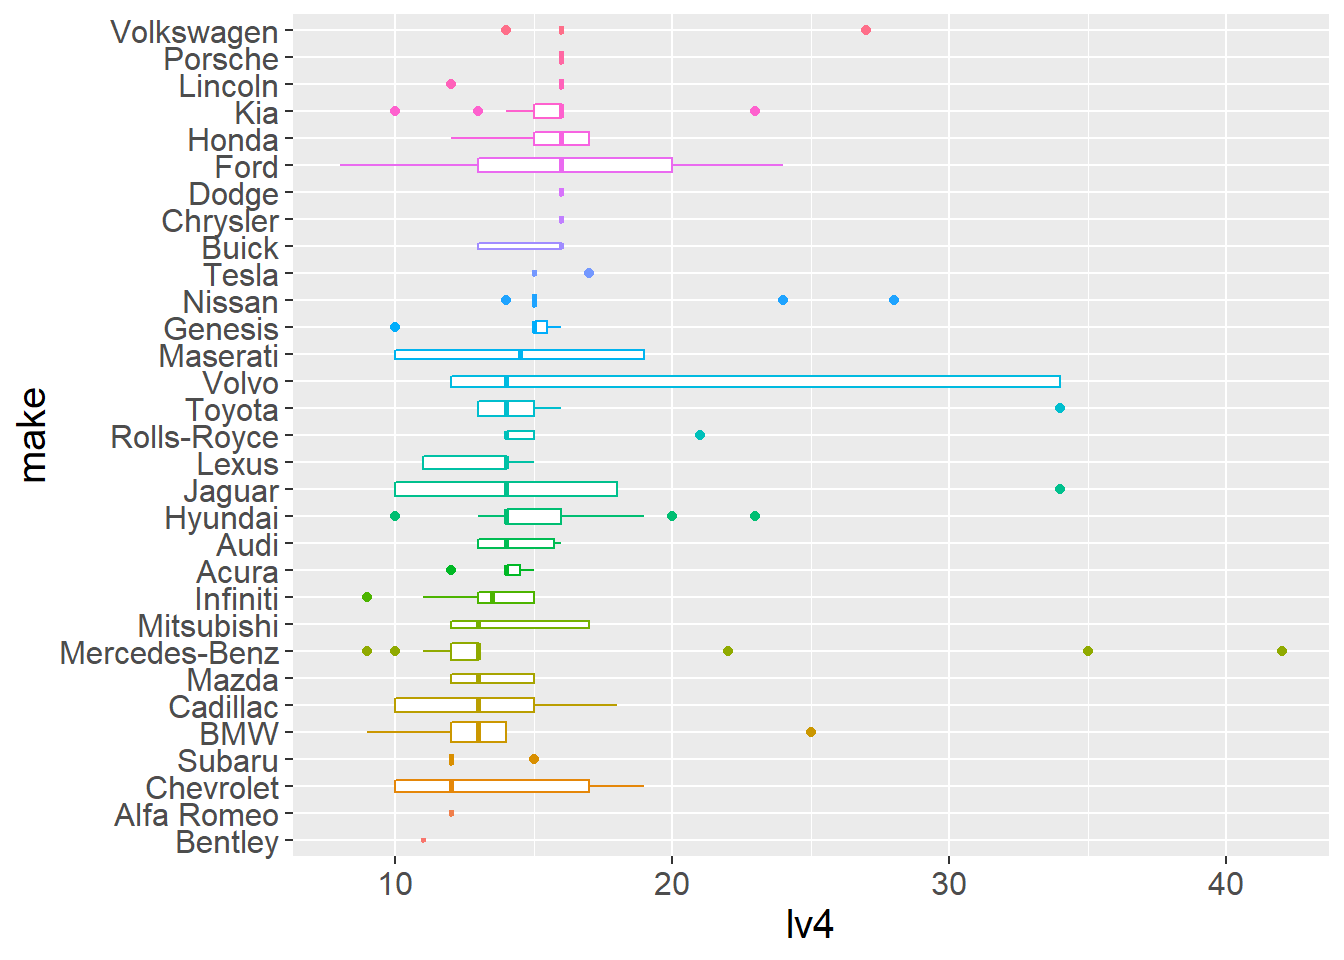
\includegraphics{2019-10-23-tidytuesday-which-are-the-best-family-cars_files/figure-latex/unnamed-chunk-6-1.pdf}

Mercedes AMG GLA45 is the winner with 42 cubic feet space!

Here is another presentation, for easier comparision.

\begin{Shaded}
\begin{Highlighting}[]
\CommentTok{# Top family cars - geom_Col()}
\NormalTok{bs_col <-}\StringTok{ }\NormalTok{boot_space }\OperatorTok\StringTok{ }
\StringTok{    }\KeywordTok{mutate}\NormalTok{(}\DataTypeTok{model =} \KeywordTok{fct_reorder}\NormalTok{(model, lv4)) }\OperatorTok
\StringTok{    }\KeywordTok{mutate}\NormalTok{(}\DataTypeTok{make =} \KeywordTok{fct_reorder}\NormalTok{(make, lv4)) }\OperatorTok\StringTok{ }
\StringTok{    }\KeywordTok{ggplot}\NormalTok{(}\KeywordTok{aes}\NormalTok{(}\DataTypeTok{x=}\NormalTok{model, }\DataTypeTok{y=}\NormalTok{lv4, }\DataTypeTok{fill=}\NormalTok{make)) }\OperatorTok{+}\StringTok{ }
\StringTok{    }\KeywordTok{geom_col}\NormalTok{(}\DataTypeTok{position=}\StringTok{"dodge"}\NormalTok{)}\OperatorTok{+}\KeywordTok{coord_flip}\NormalTok{() }\OperatorTok{+}\StringTok{ }
\StringTok{    }\KeywordTok{theme}\NormalTok{(}\DataTypeTok{plot.caption=}\KeywordTok{element_text}\NormalTok{(}\DataTypeTok{size=}\DecValTok{11}\NormalTok{), }\DataTypeTok{text =} \KeywordTok{element_text}\NormalTok{(}\DataTypeTok{size=}\DecValTok{18}\NormalTok{), }\DataTypeTok{plot.title =} \KeywordTok{element_text}\NormalTok{(}\DataTypeTok{size=}\DecValTok{32}\NormalTok{))  }\OperatorTok{+}
\KeywordTok{labs}\NormalTok{(}\DataTypeTok{caption=} \StringTok{"Data source: https://fueleconomy.gov"}\NormalTok{, }\DataTypeTok{size=}\StringTok{"Luggage Vol}\CharTok{\textbackslash{}n}\StringTok{(Cubic feet)"}\NormalTok{, }\DataTypeTok{x =} \KeywordTok{element_blank}\NormalTok{(), }\DataTypeTok{y =} \StringTok{"Luggage Vol (Cubic feet)"}\NormalTok{, }\DataTypeTok{title =} \StringTok{"Which are the best family cars?"}\NormalTok{) }\OperatorTok{+}
\StringTok{    }\KeywordTok{scale_size}\NormalTok{(}\DataTypeTok{range=}\KeywordTok{c}\NormalTok{(}\DecValTok{2}\NormalTok{, }\DecValTok{9}\NormalTok{)) }
\NormalTok{bs_col}
\end{Highlighting}
\end{Shaded}

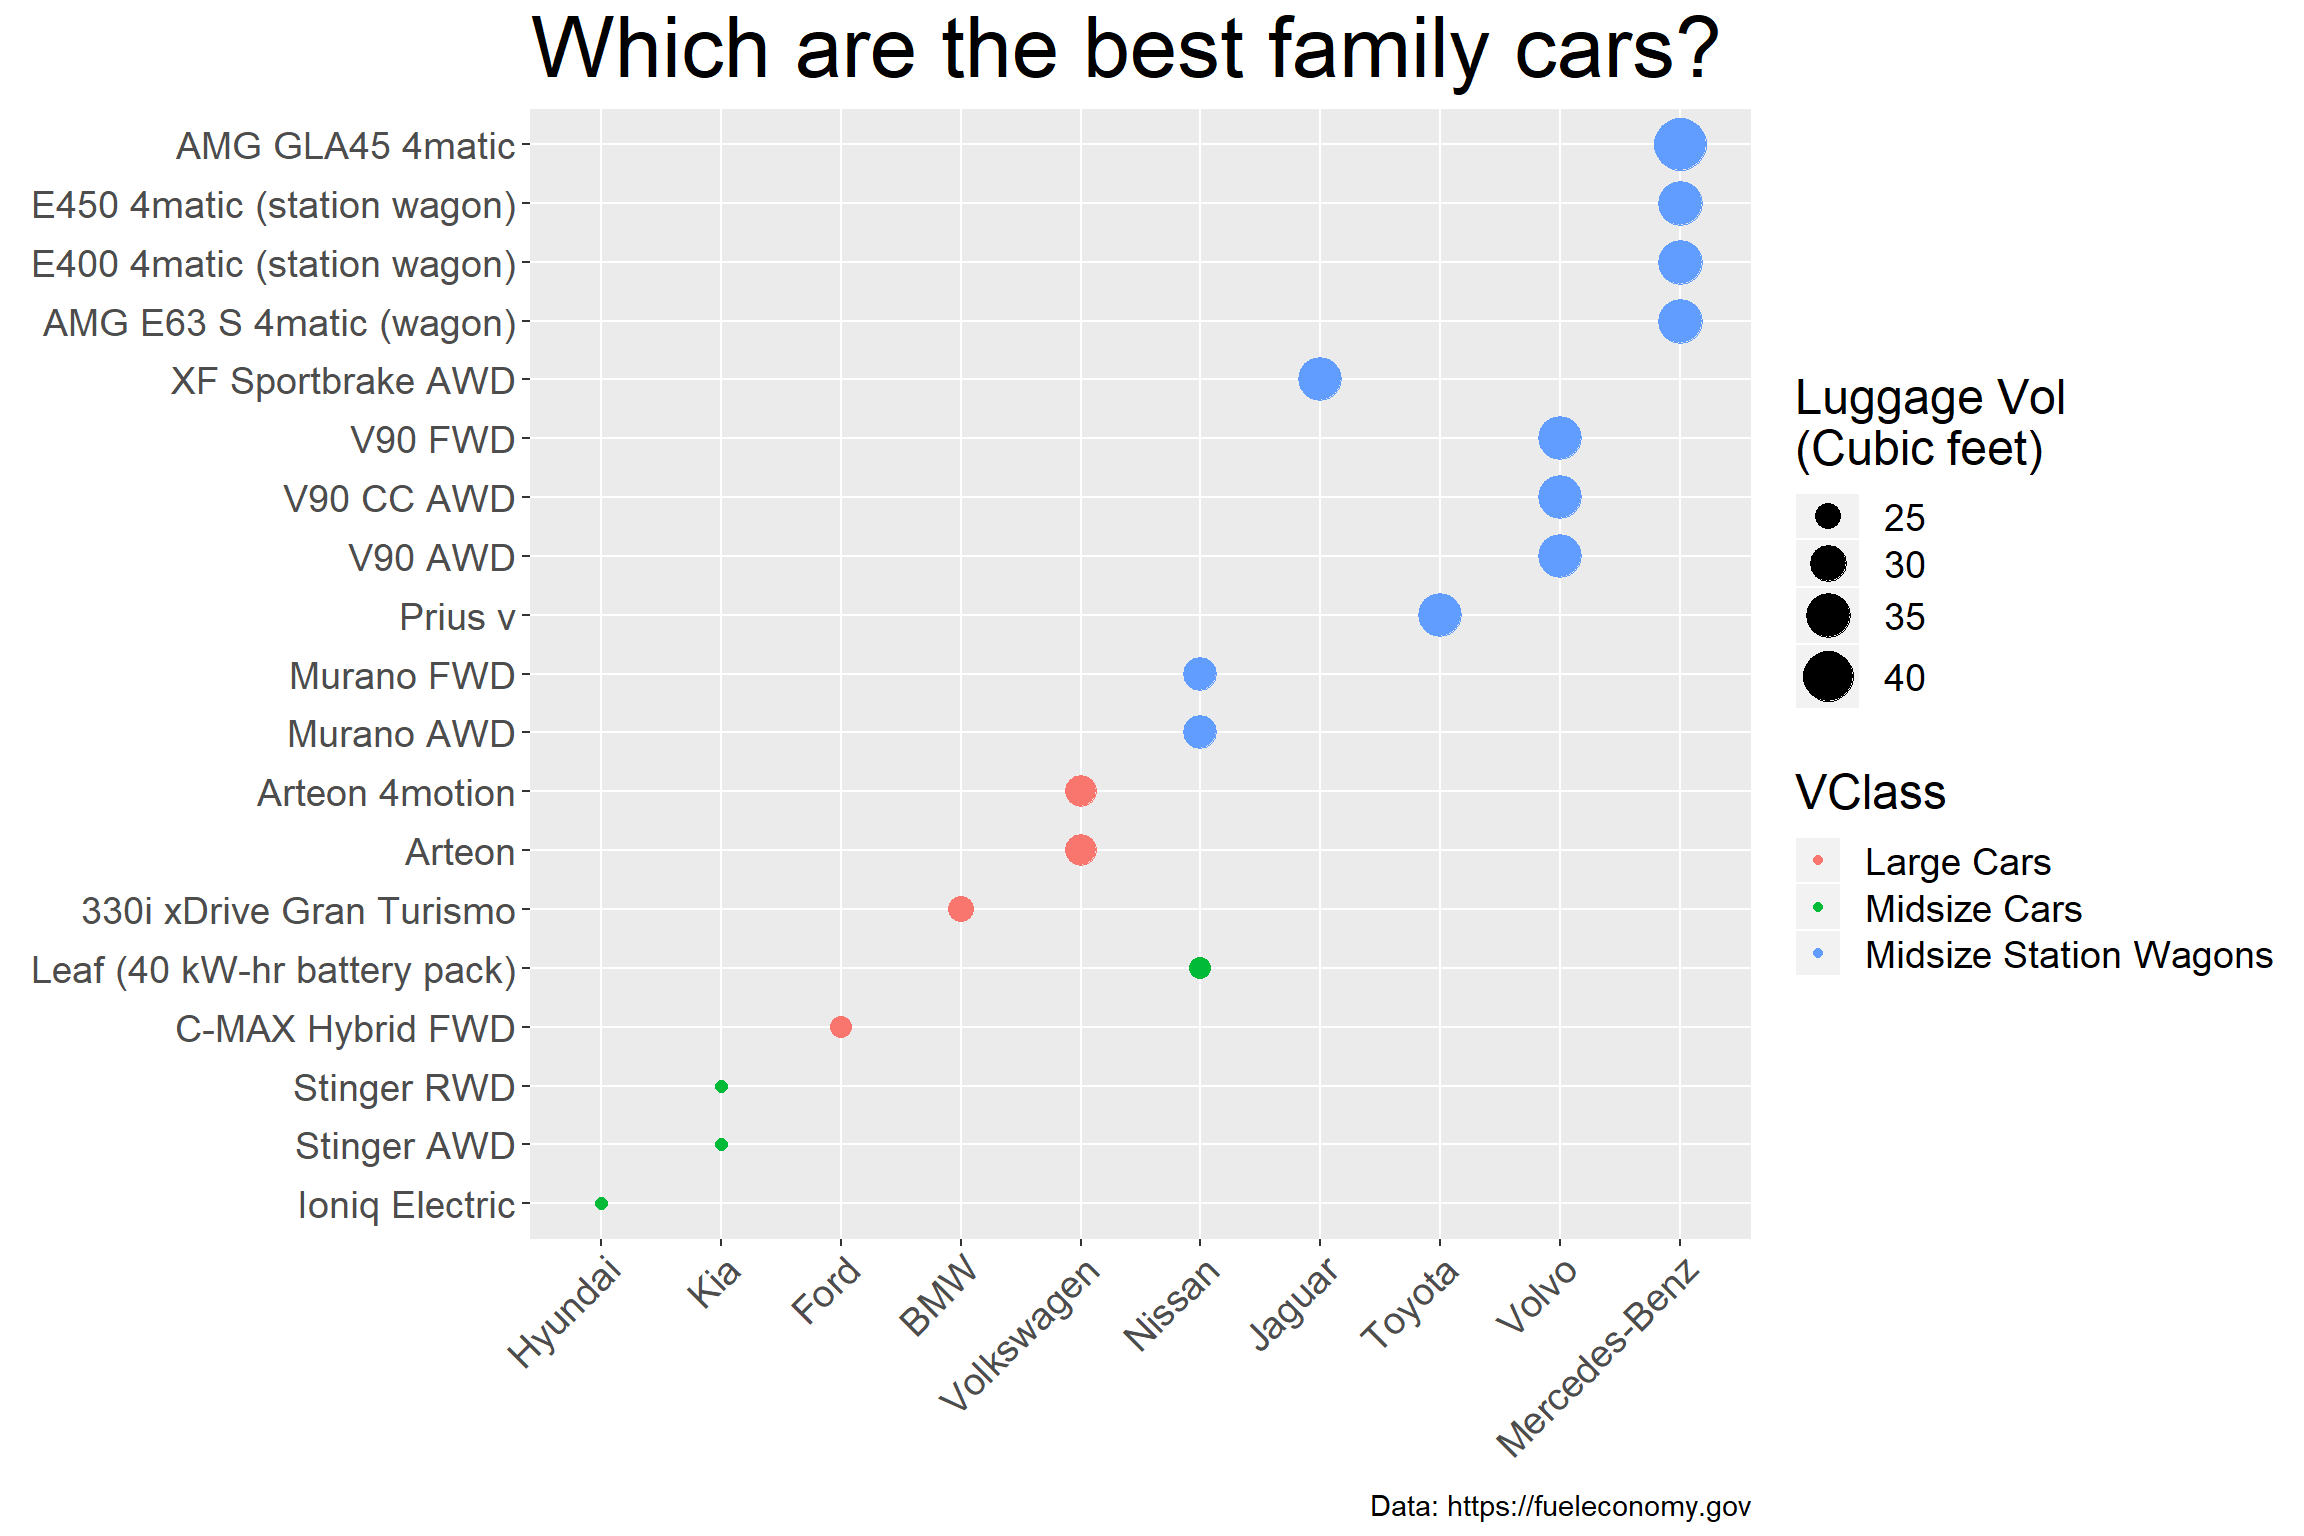
\includegraphics{2019-10-23-tidytuesday-which-are-the-best-family-cars_files/figure-latex/unnamed-chunk-7-1.pdf}

We found our answer and our camping gear is ready. Let's tackle some
other questions. We hear a lot about them but how does the future looks
like for Electric cars?

\hypertarget{how-does-electric-cars-evolving-in-the-last-years-compared-to-non-electric-cars}{%
\section{How does Electric cars evolving in the last years compared to
non electric
cars?}\label{how-does-electric-cars-evolving-in-the-last-years-compared-to-non-electric-cars}}

There are many of different types of engines capable of using one or two
different fuel sources. Let's look at how their numbers compare during
the last years.

\begin{Shaded}
\begin{Highlighting}[]
\CommentTok{# Using Varwidth: Ordered}
\NormalTok{pp  <-}\StringTok{ }\NormalTok{big_epa_cars }\OperatorTok\StringTok{ }
\StringTok{  }\KeywordTok{mutate}\NormalTok{(}\DataTypeTok{fuelType=}\KeywordTok{fct_reorder}\NormalTok{(fuelType, year)) }\OperatorTok\StringTok{ }
\StringTok{  }\KeywordTok{ggplot}\NormalTok{(}\KeywordTok{aes}\NormalTok{(}\DataTypeTok{x=}\NormalTok{fuelType, }\DataTypeTok{y =}\NormalTok{year, }\DataTypeTok{fill=}\NormalTok{fuelType)) }\OperatorTok{+}\StringTok{ }
\StringTok{  }\KeywordTok{geom_boxplot}\NormalTok{(}\DataTypeTok{varwidth=}\OtherTok{TRUE}\NormalTok{) }\OperatorTok{+}\StringTok{ }\KeywordTok{theme}\NormalTok{(}\DataTypeTok{axis.text.x =} \KeywordTok{element_text}\NormalTok{(}\DataTypeTok{angle =} \DecValTok{45}\NormalTok{, }\DataTypeTok{hjust =} \DecValTok{1}\NormalTok{)) }\OperatorTok{+}
\StringTok{  }\KeywordTok{coord_flip}\NormalTok{() }\OperatorTok{+}\StringTok{ }
\StringTok{  }\KeywordTok{theme}\NormalTok{(}\DataTypeTok{legend.position =} \StringTok{"none"}\NormalTok{, }\DataTypeTok{text =} \KeywordTok{element_text}\NormalTok{(}\DataTypeTok{size=}\DecValTok{18}\NormalTok{), }
        \DataTypeTok{plot.title =} \KeywordTok{element_text}\NormalTok{(}\DataTypeTok{size=}\DecValTok{32}\NormalTok{)) }\OperatorTok{+}\StringTok{ }
\StringTok{  }\KeywordTok{labs}\NormalTok{(}\DataTypeTok{x =} \StringTok{"Fuel Type"}\NormalTok{, }\DataTypeTok{y =} \StringTok{"Year"}\NormalTok{, }\DataTypeTok{title =} \StringTok{"How does prominence of Fuel Types }\CharTok{\textbackslash{}n}\StringTok{change with the year?"}\NormalTok{)}
\NormalTok{pp}
\end{Highlighting}
\end{Shaded}

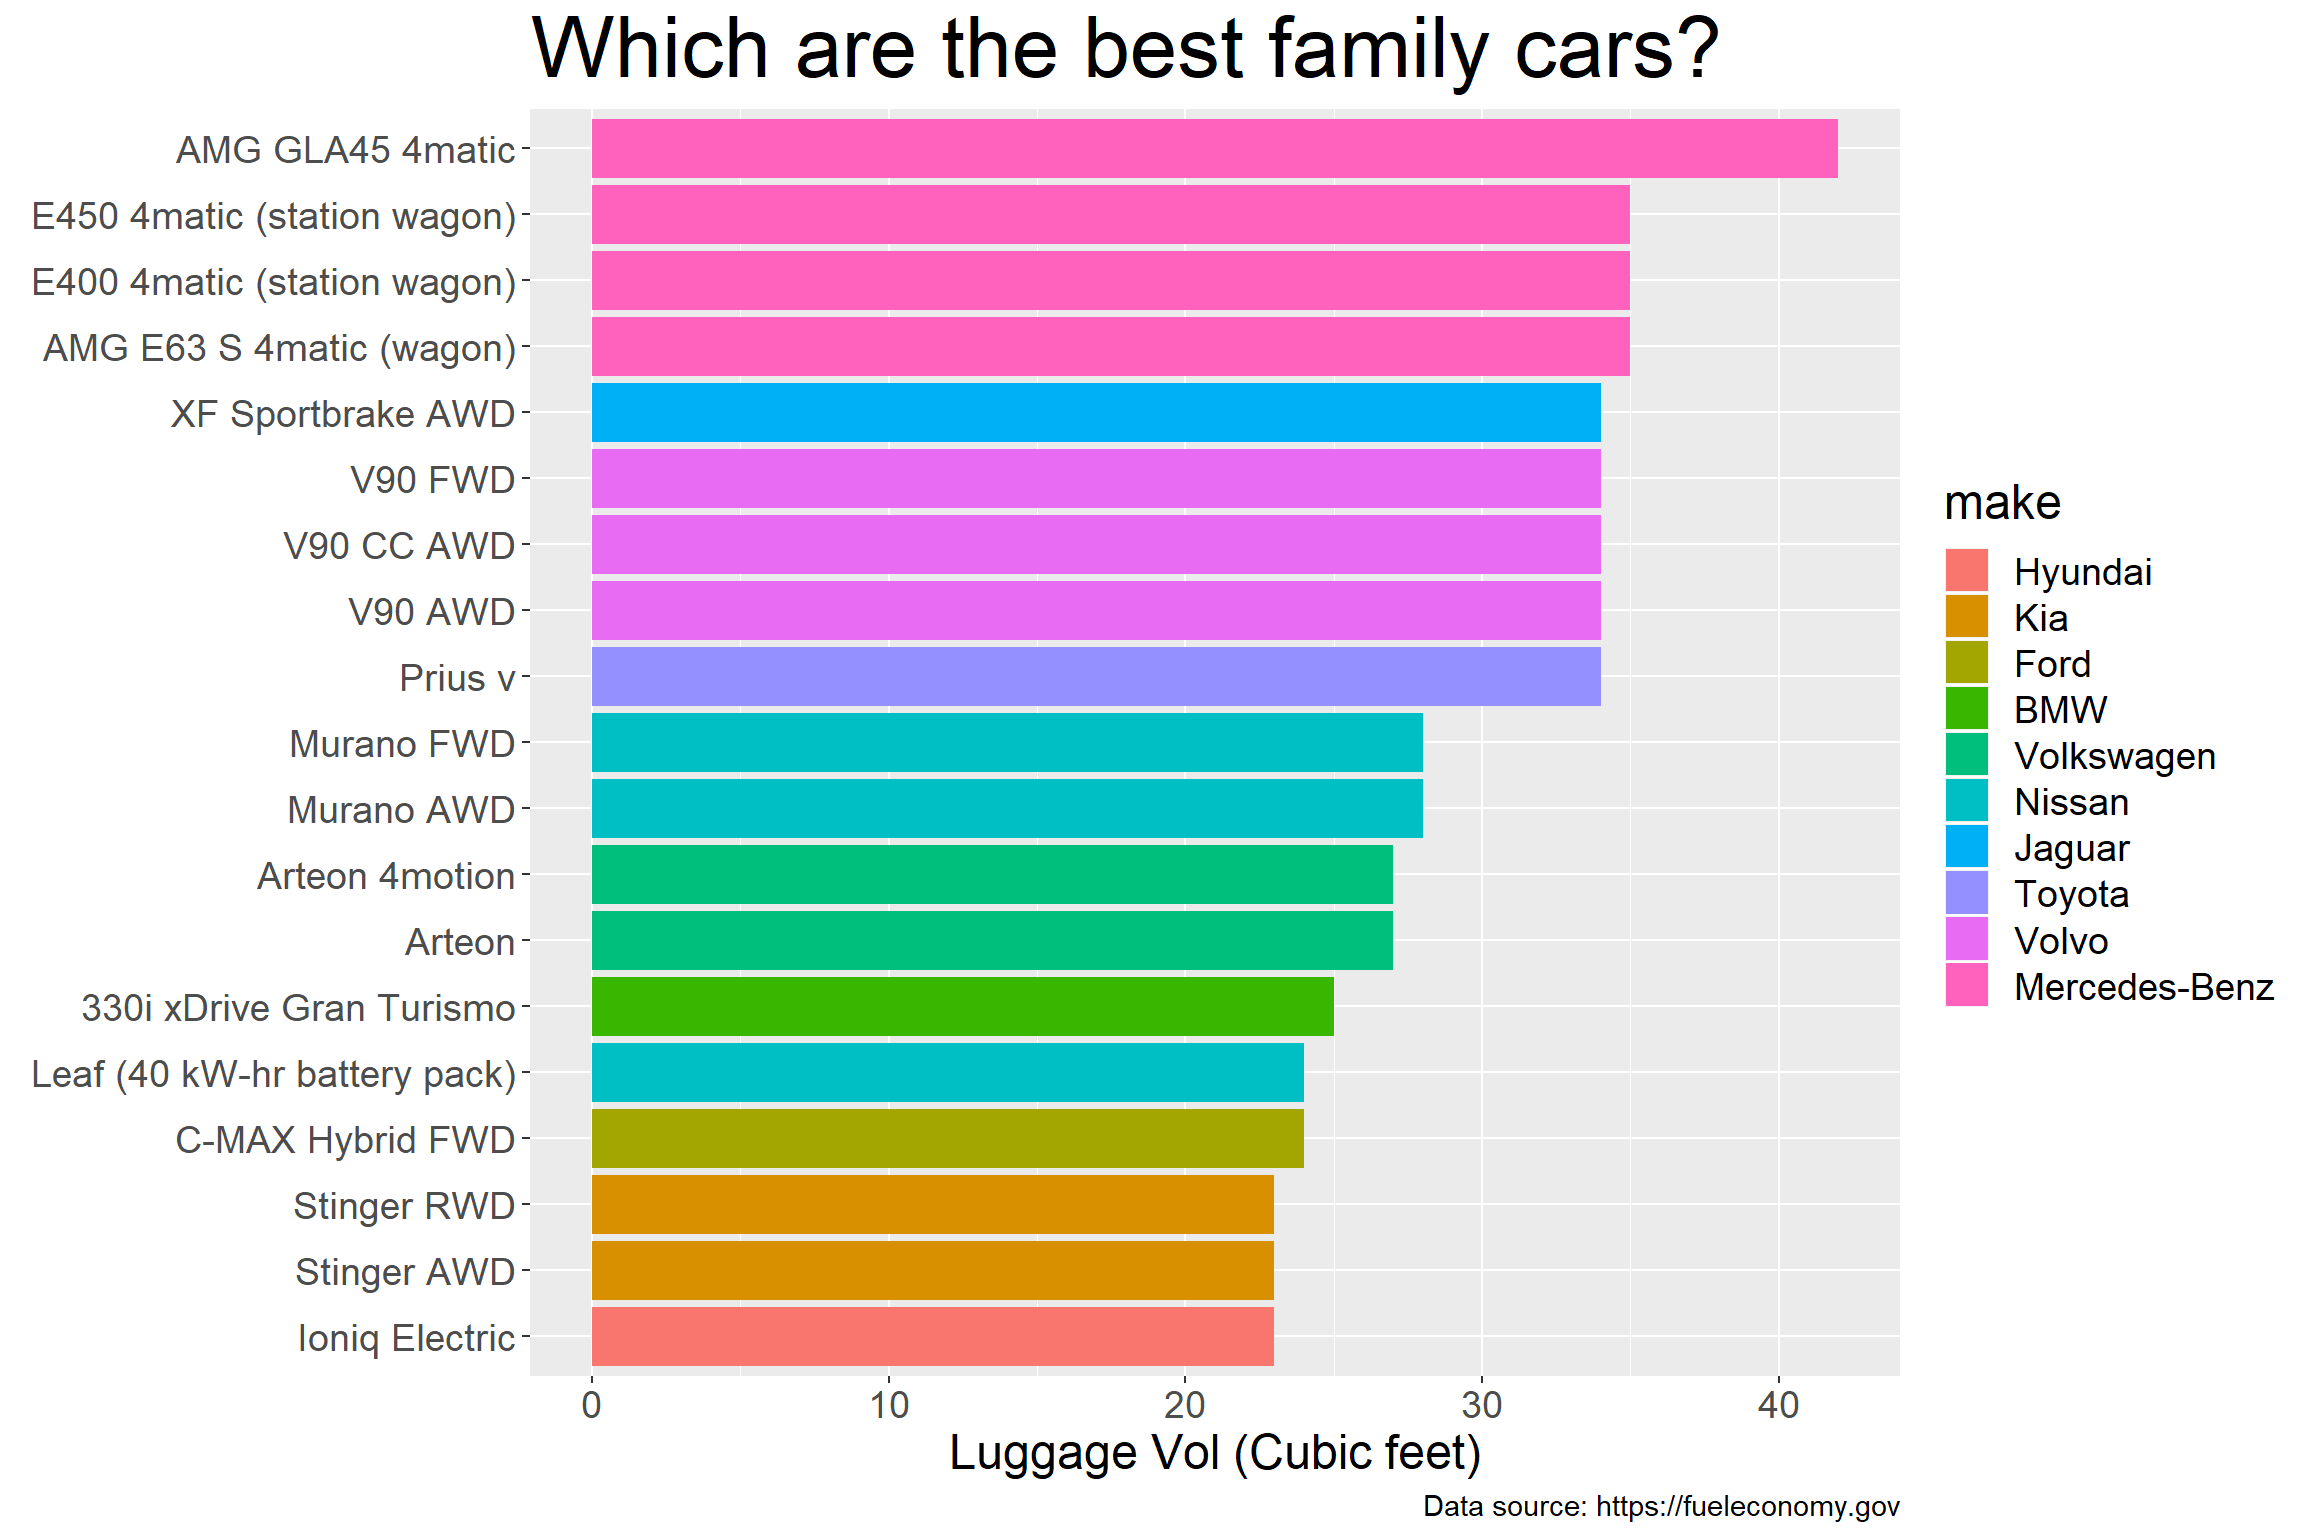
\includegraphics{2019-10-23-tidytuesday-which-are-the-best-family-cars_files/figure-latex/unnamed-chunk-8-1.pdf}

\hypertarget{group-electric-vs-non-electric-cars}{%
\subsubsection{Group Electric vs Non Electric
cars}\label{group-electric-vs-non-electric-cars}}

I will group cars according to which can use electricity vs which can't.

\begin{Shaded}
\begin{Highlighting}[]
\CommentTok{# Grouped: Electric vs no electric:}
\NormalTok{big_epa_cars}\OperatorTok{$}\NormalTok{fuelType <-}\StringTok{ }\KeywordTok{ifelse}\NormalTok{( big_epa_cars}\OperatorTok{$}\NormalTok{fuelType }\OperatorTok\StringTok{ }\KeywordTok{c}\NormalTok{(}\StringTok{"Regular Gas and Electricity"}\NormalTok{, }\StringTok{"Premium Gas or Electricity"}\NormalTok{, }\StringTok{"Premium and Electricity"}\NormalTok{, }\StringTok{"Regular Gas or Electricity"}\NormalTok{, }\StringTok{"Electricity"}\NormalTok{), }\StringTok{"Electric"}\NormalTok{, }\StringTok{"Non-Electric"}\NormalTok{)}

\NormalTok{pp  <-}\StringTok{ }\NormalTok{big_epa_cars }\OperatorTok\StringTok{ }
\StringTok{  }\KeywordTok{mutate}\NormalTok{(}\DataTypeTok{fuelType=}\KeywordTok{fct_reorder}\NormalTok{(fuelType, year)) }\OperatorTok\StringTok{ }
\StringTok{  }\KeywordTok{ggplot}\NormalTok{(}\KeywordTok{aes}\NormalTok{(}\DataTypeTok{x=}\NormalTok{fuelType, }\DataTypeTok{y =}\NormalTok{year, }\DataTypeTok{fill=}\NormalTok{fuelType)) }\OperatorTok{+}\StringTok{ }
\StringTok{  }\KeywordTok{geom_boxplot}\NormalTok{(}\DataTypeTok{varwidth=}\OtherTok{TRUE}\NormalTok{) }\OperatorTok{+}
\StringTok{  }\KeywordTok{coord_flip}\NormalTok{() }\OperatorTok{+}\StringTok{ }
\StringTok{  }\KeywordTok{theme}\NormalTok{(}\DataTypeTok{text =} \KeywordTok{element_text}\NormalTok{(}\DataTypeTok{size=}\DecValTok{18}\NormalTok{), }
        \DataTypeTok{plot.title =} \KeywordTok{element_text}\NormalTok{(}\DataTypeTok{size=}\DecValTok{32}\NormalTok{), }\DataTypeTok{legend.position =} \StringTok{"none"}\NormalTok{)}\OperatorTok{+}
\StringTok{  }\KeywordTok{theme}\NormalTok{(}\DataTypeTok{text =} \KeywordTok{element_text}\NormalTok{(}\DataTypeTok{size=}\DecValTok{15}\NormalTok{)) }\OperatorTok{+}
\StringTok{  }\KeywordTok{labs}\NormalTok{(}\DataTypeTok{x =} \StringTok{"Fuel Type"}\NormalTok{, }\DataTypeTok{y =} \StringTok{"Year"}\NormalTok{, }\DataTypeTok{title =} \StringTok{"How does prominence of Fuel Types }\CharTok{\textbackslash{}n}\StringTok{change with the year?"}\NormalTok{)}
\NormalTok{pp}
\end{Highlighting}
\end{Shaded}

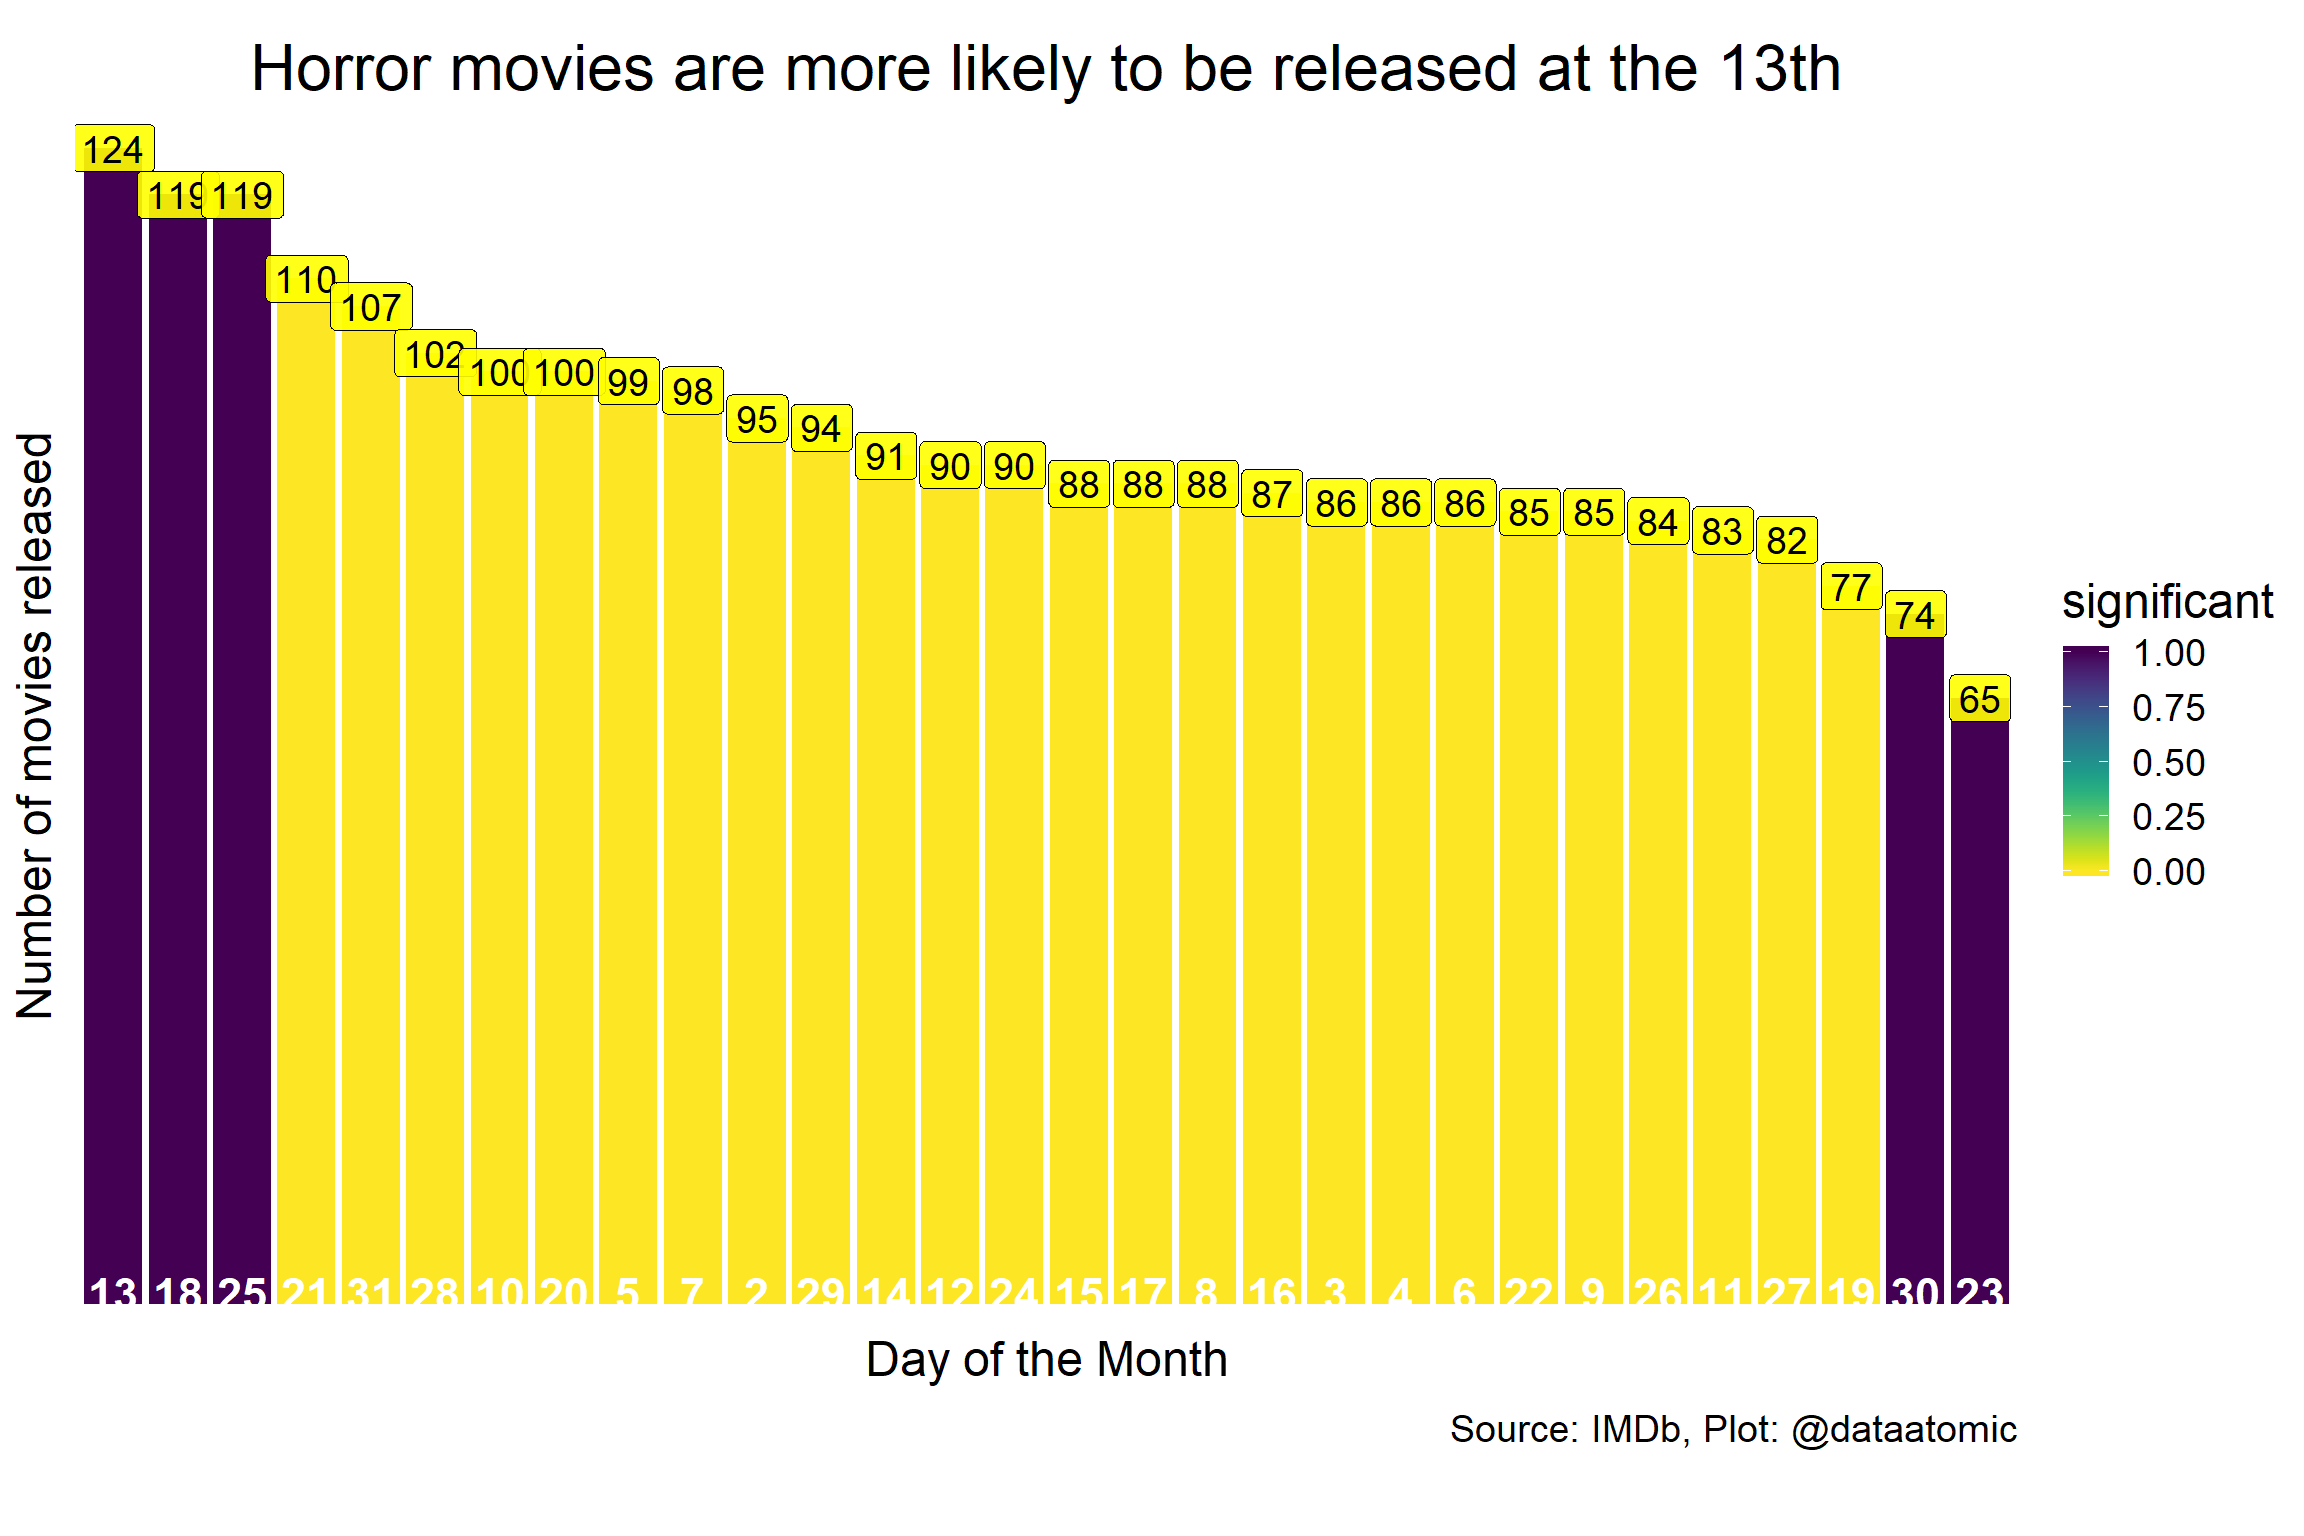
\includegraphics{2019-10-23-tidytuesday-which-are-the-best-family-cars_files/figure-latex/unnamed-chunk-9-1.pdf}

In the last couple of years, number of electric car models are
increasing but they are still a minority.

\begin{Shaded}
\begin{Highlighting}[]
\NormalTok{big3 <-}\StringTok{ }\NormalTok{big_epa_cars }\OperatorTok\StringTok{ }\KeywordTok{group_by}\NormalTok{(year, fuelType) }\OperatorTok\StringTok{ }\KeywordTok{mutate}\NormalTok{(}\DataTypeTok{n =} \KeywordTok{n}\NormalTok{())}

\NormalTok{big3 }\OperatorTok\StringTok{ }
\StringTok{    }\KeywordTok{ggplot}\NormalTok{(}\KeywordTok{aes}\NormalTok{(}\DataTypeTok{x=}\NormalTok{n, }\DataTypeTok{y =}\NormalTok{year, }\DataTypeTok{col=}\NormalTok{fuelType)) }\OperatorTok{+}
\StringTok{    }\KeywordTok{geom_point}\NormalTok{(}\DataTypeTok{size=}\DecValTok{4}\NormalTok{) }\OperatorTok{+}
\StringTok{    }\KeywordTok{theme}\NormalTok{(}\DataTypeTok{legend.position =} \KeywordTok{c}\NormalTok{(}\FloatTok{0.9}\NormalTok{,}\FloatTok{0.9}\NormalTok{), }\DataTypeTok{legend.title=} \KeywordTok{element_blank}\NormalTok{(), }\DataTypeTok{legend.background =} \KeywordTok{element_blank}\NormalTok{()) }\OperatorTok{+}\StringTok{ }
\StringTok{    }\KeywordTok{theme}\NormalTok{(}\DataTypeTok{plot.title =} \KeywordTok{element_text}\NormalTok{(}\DataTypeTok{size=}\DecValTok{32}\NormalTok{), }\DataTypeTok{text =} \KeywordTok{element_text}\NormalTok{(}\DataTypeTok{size=}\DecValTok{15}\NormalTok{)) }\OperatorTok{+}\StringTok{ }\KeywordTok{coord_flip}\NormalTok{() }\OperatorTok{+}
\StringTok{    }\KeywordTok{labs}\NormalTok{(}\DataTypeTok{x =} \StringTok{"Number of Car models"}\NormalTok{, }\DataTypeTok{y =} \StringTok{"Year"}\NormalTok{, }\DataTypeTok{title =} \StringTok{"How does the Numbers of Electric vs Non Electric cars }\CharTok{\textbackslash{}n}\StringTok{change by year?"}\NormalTok{)}
\end{Highlighting}
\end{Shaded}

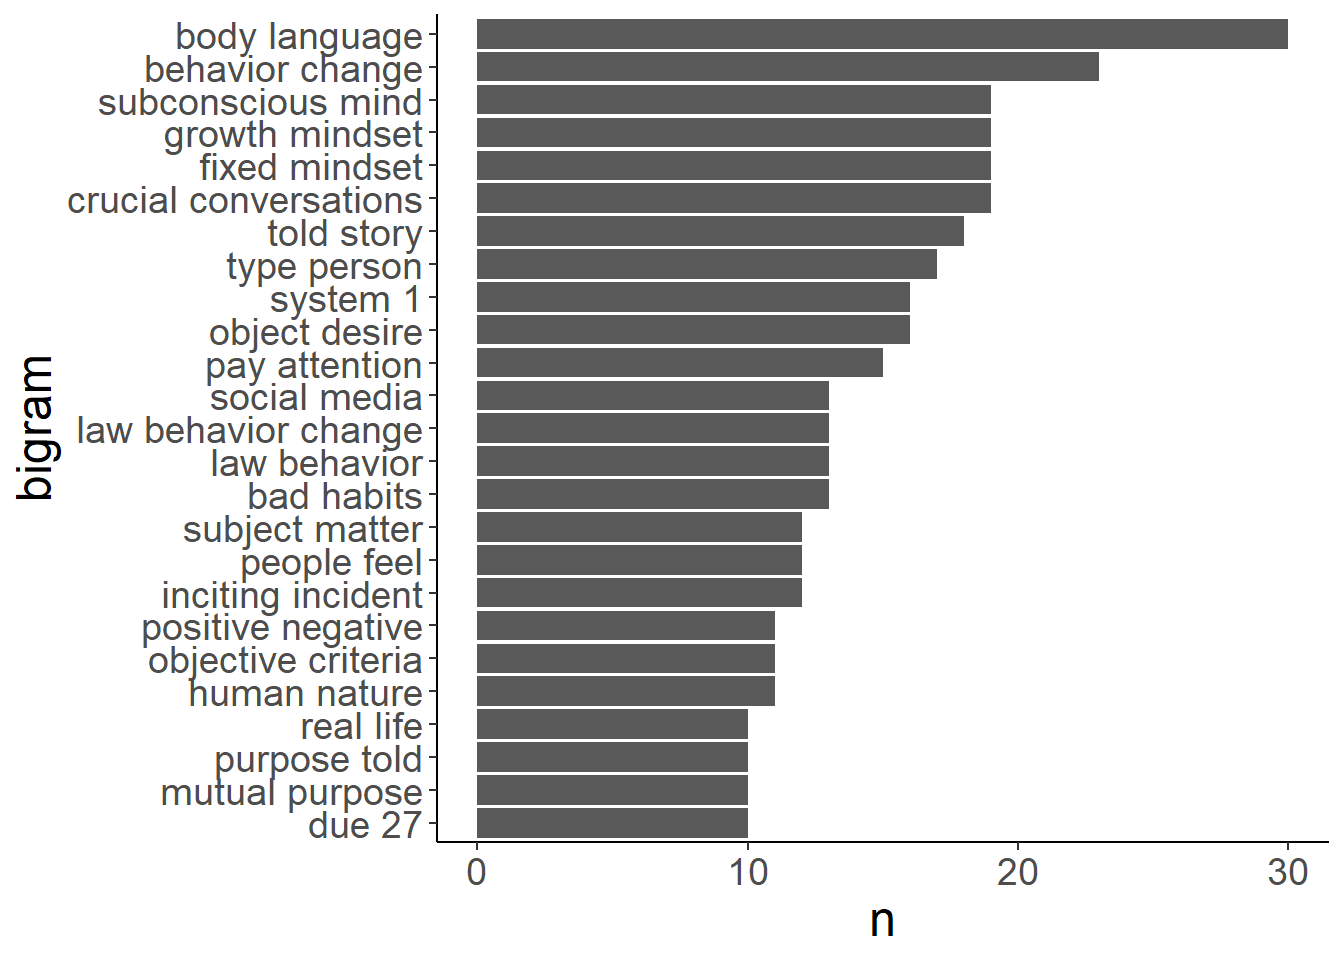
\includegraphics{2019-10-23-tidytuesday-which-are-the-best-family-cars_files/figure-latex/unnamed-chunk-10-1.pdf}

Both Electric and Non Electric car models follows a similar increase in
the last 10 years

Increases in Electric car models in the last years might be a reflection
of a general increase in total number of model types

\hypertarget{conclusions-future-thoughts}{%
\section{Conclusions / Future
thoughts}\label{conclusions-future-thoughts}}

This was a huge dataset. You can answer other questions such as mileage
of different car models, carbon dioxide emissions, fuel savings and many
more.

I have selected some car models which might be a good option if luggage
space is a priority for you!

To see other examples of how people used this dataset follow the
\href{https://twitter.com/hashtag/tidytuesday?lang=en}{Twitter hashtag
\#TidyTuesday}.

Please share if you have other ideas in the comments below!

Until next time!

Serdar


\end{document}
